\documentclass{article}
\usepackage{amsmath}
\usepackage{amssymb}
\usepackage{graphicx}
\usepackage{hyperref}
\usepackage[version=4]{mhchem}

\title{Example 4}
\date{}

\begin{document}
\maketitle

In \(\triangle A B C\), the angle bisector of \(\angle A\) meets \(B C\) at \(D\). Show that \(A D^{2}=A B \cdot A C-B D \cdot C D\).

Solution:
Construct a circle that circumscribes the triangle as shown in the figure. Extend \(A D\) to meet the circle at \(E\) and connect \(B E\).\\
\centering
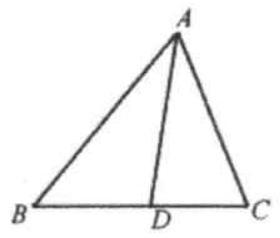
\includegraphics[width=\textwidth]{images/problem_image_1.jpg}

Since \(\angle E=\angle C\) (both face the same \(\operatorname{arc} A B) . \angle 1=\angle 2\), \(\triangle A B E \sim \triangle A D C\)\\
\(A B \cdot A C=A D \cdot A E\)\\
\(B D \cdot D C=A D \cdot D E\)\\
(1) \(-(2):\)\\
\centering
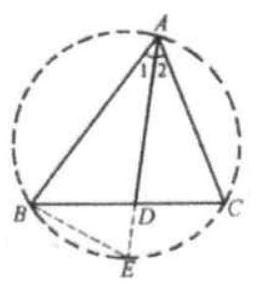
\includegraphics[width=\textwidth]{images/reasoning_image_1.jpg}\\
\(A B \cdot A C-B D \cdot C D=A D \cdot A E-A D \cdot D E\)\\
\(=A D(A E-D E)=A D \cdot A D=A D^{2}\)\\
Therefore \(A D^{2}=A B \cdot A C-B D \cdot C D\).


\end{document}
